%!TEX root = ../thesis.tex
%*******************************************************************************
%****************************** Second Chapter *********************************
%*******************************************************************************

\chapter{Modelos predictivos asociados a mutaciones puntuales en proteínas \label{cap2}}

\ifpdf
    \graphicspath{{Chapter2/Figs/Raster/}{Chapter2/Figs/PDF/}{Chapter2/Figs/}}
\else
    \graphicspath{{Chapter2/Figs/Vector/}{Chapter2/Figs/}}
\fi

El análisis del efecto de mutaciones puntuales en proteínas, es una de las problemáticas más estudiadas en los últimos años. Las investigaciones se enfocan principalmente en la evaluación de cambios en la estabilidad de la proteína mediante la variación de energía libre que la mutación provoca \cite{Schymkowitz2005,Pandurangan2017,rohl2004protein,Parthiban2006}. 

Diferentes modelos predictivos han sido desarrollados para poder predecir cambios de energía libre, en base a algoritmos de aprendizaje supervisado o mediante técnicas de minería de datos y así, determinar el efecto de la mutación en set de proteínas de interés \cite{Quan2016,Capriotti2008,Broom2017,Khan2010,vaisman,Getov2016,Capriotti2005}. No obstante, en casos más específicos, se han desarrollado modelos para proteínas independientes, con el fin de asociar la mutación a un rasgo clínico, particularmente, enfocado a casos de cáncer \cite{article, Forbes2010}, cambios en termo estabilidad \cite{Tian2010}, propiedades geométricas \cite{Barenboim2008}, entre las principales.

Sin importar el uso o la respuesta de los modelos, es necesario construir set de datos con ejemplos etiquetados, es decir, cuya respuesta sea conocida para poder entrenar modelos basados en algoritmos de aprendizaje supervisado y así evaluar su desempeño. Los enfoques principales al desarrollo de descriptores se basan en propiedades fisicoquímicas y termodinámicas, así como también, el ambiente bajo el cual se encuentra la mutación \cite{Capriotti2005}, ya sea a partir de la información estructural o sólo considerando la secuencia lineal. Sin embargo, no son considerados, los componentes asociados a conceptos filogenéticos y la propensión a cambios de dicha mutación, generando un gap entre ambos puntos de vista \cite{Olivera-Nappa2011}.

Dado a los modelos existentes y en vista a la necesidad de generar nuevos sistemas de predicción para mutaciones puntuales en proteínas, en respuesta al aumento considerable de reportes en los últimos años, se propone una nueva metodología para el diseño e implementación de modelos predictivos en mutaciones puntuales de proteínas.

Las mutaciones son descritas desde los puntos de vista estructural, termodinámico y filogenético. El desarrollo de los predictores es inspirado en el concepto de Meta Learning y es apoyado con técnicas estadísticas, tanto para la selección de modelos como para la evaluación de medidas de desempeño, entregando como resultado, un conjunto de modelos para las mutaciones puntuales reportadas, unificados en un único meta modelo.

Esta metodología será aplicada para generar estimadores en diferentes proteínas con mutaciones reportadas con respuesta conocida, como por ejemplo: evaluando las diferencias de energía libre que provoca la mutación y clasificaciones para evaluar si la sustitución de residuos aumenta o disminuye la estabilidad. A su vez, se implementarán modelos de clasificación para determinar la propensión clínica en un conjunto de mutaciones conocidas relacionados con el gen \textit{p}VHL, responsable de la enfermedad von Hippel-Lindau, con el fin de exponer la versatilidad de la metodología y los problemas relevantes a set de datos altamente no-lineales.

A continuación, se describen los principales conceptos relacionados a aprendizaje supervisado, seguido de algunas herramientas computacionales para el análisis de mutaciones y su relevancia en la de estabilidad de una proteína, continuando con la metodología propuesta, la caracterización de los diferentes set de datos a utilizar y resultados parciales obtenidos al aplicar esta metodología.

\section{Aprendizaje de Máquinas}

Aprendizaje de Máquina, es una rama de la inteligencia artificial que tiene por objetivo el desarrollo de técnicas que permitan a los computadores aprender, es decir, generalizar comportamientos a partir de una información no estructurada suministrada en forma de ejemplos \cite{michie1994machine}. Aplicándose en diferentes campos de investigación: motores de búsqueda \cite{cooley1997web}, diagnósticos médicos \cite{7912315,ABDELAZIZ2018117}, detección de fraude en el uso de tarjetas de crédito, bioinformática \cite{juanito}, reconocimiento de patrones en imágenes \cite{imageA} y textos \cite{netzer2011reading,alm2005emotions}, etc. 

Los algoritmos de aprendizaje pueden clasificarse en dos grandes grupos \cite{michie1994machine}:

\begin{itemize}
	
	\item \textbf{Supervisados}: se cumple un rol de predicción, clasificación, asignación, etc. a un conjunto de elementos con características similares, por lo que los datos de entrada son conocidos.
	
	\item \textbf{No Supervisados}: su objetivo es agrupar en conjuntos con características similares los elementos de entrada dado los valores de estos atributos, en base a la asociación de patrones característicos que representen sus comportamientos.
\end{itemize}

A continuación se describen en forma general, los algoritmos de aprendizaje supervisados utilizados para el desarrollo de la metodología, explicando los conceptos bajo los que se basan y cómo estos entrenan y se emplean para predecir o clasificar nuevos ejemplos.

\subsection{Algoritmos de aprendizaje supervisado}

Existen diferentes algoritmos de aprendizaje supervisado, los cuales pueden ser asociados a la clasificación de un elemento o la predicción de valores, dependiendo el tipo de respuesta existente en el conjunto de datos a estudiar. En el caso de respuestas con distribución continua, se trabajan con algoritmos de regresión, mientras que si la respuesta es binaria o multiclase y es representada por variables categóricas, los algoritmos se basan en clasificadores \cite{michie1994machine}.

A su vez, también se pueden dividir con respecto a la forma en que se trata el problema, existiendo algoritmos basados en cálculos de distancia entre ejemplos (K-Vecinos Cercanos), otros que consideran transformaciones vectoriales y aplicaciones de funciones de kernel (Máquina Soporte de Vectores), así como también el uso de las características como entorno espacial de decisión (Árboles y métodos de ensamble) y aquellos que utilizan redes neuronales y trabajan en torno a cajas negras, o métodos basados en regresiones lineales, sólo aplicados a modelos predictivos de variables continuas.

Cada uno de estos algoritmos es descrito a continuación, enfocándose tanto en el componente matemático asociado, así como también en las ventajas y usos posibles que estos puedan tener, con respecto al conjunto de datos a trabajar.

\subsection{Métodos basados en regresiones lineales}

Regresión lineal, es uno de los métodos más simples en cuanto a predicción de variables continuas, además de uno de los más limitantes debido al sobreajuste que éste puede generar. No obstante, permite evaluar de manera simple y sencilla conjuntos de datos \cite{graybill1976theory}. 

Matemáticamente, se espera que el conjunto de respuesta sea el resultado de una combinación lineal de parámetros, es decir. Sea $\hat{y}$ el vector de predicciones, se tiene que:

\begin{equation}
	\hat{y}(w, x) = w_0 + w_1 x_1 + ... + w_p x_p
\end{equation}

Donde $w_0$ es el intercepto y $w = (w_1,\cdots, w_p)$ el vector de coeficientes.

Existente diferentes métodos de regresión lineal, los cuales cumplen con el mismo objetivo. Sin embargo, la forma en la que minimizan el error asociado a las diferencias entre los valores predichos y los observados.

Pese a su simplicidad, los métodos basados en regresiones lineales han sido ampliamente utilizados. No obstante, presentan diferentes problemas asociados al sobreajuste de parámetros.
 
\subsection{K-Vecinos Cercanos}

Algoritmo de aprendizaje supervisado, el cual tiene por objetivo asociar un elemento a una clase en particular, dada la información de ejemplos de entrada que tengan asociadas características particulares, que puedan declararse como \textit{vecinos} del nuevo ejemplo a clasificar, siendo \textbf{k} el número de vecinos que se está dispuesto a utilizar para aplicar la clasificación \cite{6313426}. La mejor elección de \textbf{k} depende fundamentalmente de los datos; generalmente, valores grandes de \textbf{k} reducen el efecto de ruido en la clasificación, pero crean límites entre clases parecidas.

Con el fin de evaluar la cercanía de los ejemplos existentes contra el nuevo ejemplo a clasificar, es necesario asociar ciertas medidas de distancia que permitan cuantificar esta característica, para así poder comparar esta distancia y evaluar la cercanía para asociarle una clase a este nuevo ejemplo \cite{5408784}. La distancia a emplear para evaluar la cercanía puede ser: Euclidiana \cite{DANIELSSON1980227}, Manhattan \cite{PERLIBAKAS2004711}, coseno \cite{LIAO20155328} o Mahalanobis \cite{DEMAESSCHALCK20001}, entre las principales.

\subsection{Naive Bayes}

Naive Bayes es un conjunto de algoritmos de aprendizaje supervisados basados en la aplicación del teorema de Bayes con la suposición "ingenua" de independencia entre cada par de características \cite{zhang2004optimality}. Dada una variable de clase $y$ y un vector de característica dependientes de la forma $x_1,..., x_n$ se puede utilizar la siguiente regla de clasificación:

\begin{equation}
	P(y \mid x_1, \dots, x_n) \propto P(y) \prod_{i=1}^{n} P(x_i \mid y)
\end{equation}

\begin{center}
	$\Downarrow$ 
\end{center}
\begin{equation}
	\hat{y} = \arg\max_y P(y) \prod_{i=1}^{n} P(x_i \mid y)
\end{equation}

A pesar de sus supuestos aparentemente simplificados, los clasificadores de Naive Bayes han funcionado bastante bien en muchas situaciones del mundo real, la famosa clasificación de documentos y el filtrado de spam son ejemplos de ello \cite{10.1007/BFb0026666, Chen2009, metsis2006spam}. Requieren una pequeña cantidad de datos de entrenamiento para estimar los parámetros necesarios. Pueden ser extremadamente rápido en comparación con métodos más sofisticados. 

Existen distintos tipos de clasificadores de Naive Bayes, diferenciándose entre sí en la función de distribución de probabilidad que utilizan \cite{metsis2006spam,john1995estimating,manning2010introduction}, dentro de los que se encuentran: Gaussian Naive Bayes, Multinomial Naive Bayes y Bernoulli Naive Bayes.

\subsection{Árboles de Decisión}

Se define árbol de  decisión como un modelo de predicción, utilizado en el ámbito de la inteligencia artificial, en el cual,  dado un conjunto de datos, se fabrican diagramas de construcciones lógicas, muy similares a los sistemas de predicción basados en reglas, que sirven para representar y categorizar una serie de condiciones que ocurren de forma sucesiva, para la resolución de un problema \cite{freund1999alternating}.  

El aprendizaje basado en árboles de decisión utiliza un árbol como un modelo predictivo que mapea las observaciones de las características que presenta un elemento. En estas estructuras de árbol, las hojas representan etiquetas de conjuntos ya clasificados, los nodos, a su vez, nombres o identificadores de los atributos y las ramas representan posibles valores para dichos atributos \cite{bhargava2013decision}.


Este tipo de entrenamiento, es uno de los más utilizados, debido a su simplicidad a la forma en la que trabaja, ya que, permite comprender del problema, con respecto a los atributos y cómo estos van distribuyendo las respuestas, así, es posible entender las decisiones que toma el algoritmo para clasificar o predecir nuevos ejemplos, determinar comportamientos preferentes y tendencias sobre atributos y rangos de estos.

\subsection{Support Vector Machine (SVM)}

Máquina soporte de vectores (SVM por sus siglas en inglés), es un conjunto de métodos de aprendizaje supervisado, utilizados para clasificar, predecir e inclusive para la detección de puntos outliers  \cite{scholkopf2001learning}. 

SVM genera una representación de los ejemplos como puntos en el espacio, mapeados de modo que los ejemplos de las categorías separadas se dividan por un espacio claro que es tan amplio como sea posible. Nuevos ejemplos son entonces mapeados en ese mismo espacio y predicen si pertenecen a una categoría en base a qué lado del espacio son asignados \cite{scholkopf2001learning}.

Las predicciones se realizan de manera eficiente, utilizando funciones kernel para su transformación en espacios no lineales \cite{amari1999improving}. Esto permite generar transformaciones de espacio dimensional de los datos, para mapear implícitamente sus entradas en espacios característicos de alta dimensión. 

\subsection{Métodos de ensamble}

Los métodos de ensamble, se basan en la combinación de las predicciones obtenidas por varios estimadores, construidos en base a algoritmos de aprendizaje supervisado, con el fin de mejorar la generalización del modelo y aumentar la robustez ante nuevos ejemplos \cite{dietterich2000ensemble}.

Existen dos familias de métodos de ensamble, las cuales se diferencian principalmente en la forma en que combinan los modelos para obtener la medida de desempeño final \cite{kotsiantis2007supervised}:

\begin{enumerate}
	
	\item \textbf{Métodos ponderados}: basados en la construcción de varios estimadores independientes y promediar sus medidas de desempeño, esto mejora el rendimiento debido a que disminuye la variabilidad de las clasificaciones. Ejemplos comunes de esto son Bagging y Random Forest.
	
	\item \textbf{Métodos boosting}: basados en la construcción secuencial de modelos, intentando disminuir el sesgo del modelo combinando diferentes estimadores débiles. Cumple con la filosofía \textit{"la unión de varios modelos débiles, puede construir uno fuerte"}. Ejemplos comunes de esto son AdaBoost y Gradient Tree Boosting.
	
\end{enumerate}

A continuación, se explican brevemente algunos de los algoritmos asociados a la familia de métodos de ensamble.

\subsubsection{Bagging}

Bagging forma parte de los métodos ponderados, en particular, se puede definir como métodos que forman una clase de algoritmos compuestos por varias instancias de un estimador, entrenados en base a subconjuntos aleatorios del set de datos original, ponderando sus predicciones individuales en una respuesta ponderada. El objetivo general de estos métodos es reducir la varianza de un estimador, por medio del proceso de entrenamiento de subconjuntos aleatorios \cite{breiman1996bagging}. 

\subsubsection{Random Forest \label{rf}}

Random Forest es un método de ensamble ponderado basado en árboles de decisión aleatorios. Conjuntos de diversos clasificadores son creados basados en efectos aleatorios tanto de la extracción de características como de ejemplos, formando subconjuntos de elementos, cada uno de estos aporta con un valor de estimación, el cual es ponderado con los restantes, obteniendo así, la medida general \cite{breiman1998}.

\subsubsection{AdaBoost}

AdaBoost, es un algoritmo basado en el método boosting, lo que implica que se ajusta a una secuencia de estimadores débiles obtenidos a partir de diferentes subconjuntos de datos generados de manera aleatoria desde el conjunto inicial de datos de entrenamiento \cite{CAO2013745}. 

Cada una de las predicciones obtenidas por los estimadores se combinan de manera ponderada por votación, en el caso de modelos de clasificación, o a través de un promedio en base a las estimaciones resultantes, en el caso de modelos de regresión \cite{hastie2009multi}. 

\subsubsection{Gradient Tree Boosting}

Gradient Tree Boosting o Gradient Boosted Regression Trees, es una generalización de métodos de boosting para funciones diferenciables arbitrarias de pérdida \cite{gradient}. Es un método considerado como preciso y efectivo, el cual puede usarse tanto para el desarrollo de modelos de clasificación como de regresión, siendo usado en diferentes áreas de investigación: motores de búsqueda, ecología, minerología, biotecnología, entre otros.

Dentro de las principales ventajas que posee, se encuentran: manejo natural de diferentes tipos de características en un set de datos, alto poder predictivo y robusto frente a la predicción de valores atípicos en una muestra \cite{FRIEDMAN2002367}.

\subsection{Redes Neuronales y Deep Learning}

Redes neuronales es posible definirlas como una serie de modelos de aprendizaje que se basan en la forma de trabajo de las redes neuronales biológicas, es decir, se usa el concepto de \textit{neurona} para estimar una función aproximada, la cual dependerá de un largo número de inputs, generalmente desconocidos.

En la Figura \ref{red} se aprecia un sistema de red neuronal, en la cual se observa un sistema interconectado por neuronas, las cuales intercambian información en forma de mensaje entre ellas, además cada interconexión tiene un peso, el cual es un valor numérico, que puede ser obtenido en base a la experiencia.

En resumen, una red neuronal es un conjunto de entradas y salidas regidas por capas intermedias que permiten evaluar la salida, dichas capas operan entre sí en base a funciones matemáticas y brindan un peso a la conexión, finalmente cada capa es usada para diseñar un modelo de aprendizaje supervisado o no.

\begin{figure}[!h]
	\centering
	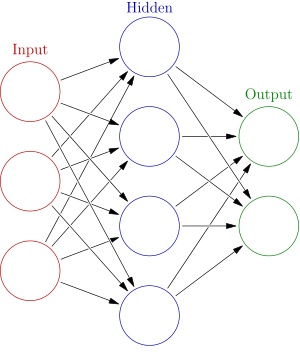
\includegraphics[scale=.5]{red.png}
	\caption{Representación esquemática de una Red Neuronal}
	\label{red}
\end{figure} 

Deep Learning es una herramienta de Machine Learning la cual tiene por objetivo modelar abstracciones de alto nivel en los datos por medio del uso de múltiples capas de procesamiento, ya sea a través del uso de estructuras complejas a través de múltiples transformaciones no lineales \cite{bengio2013representation, MAL-006, SIG-039}. 

La investigación en esta área tiene por objetivo generar mejores representaciones y crear modelos para aprender de éstas a partir de datos no marcados a gran escala. En geneal, las representaciones obtenidas se inspiran en los avances en la neurociencia y se basa libremente en la interpretación de los patrones de procesamiento y comunicación de información en un sistema nervioso, como la codificación neural que intenta definir una relación entre varios estímulos y respuestas neuronales asociadas en el cerebro \cite{MAL-006}.

Deep learning es un método específico de machine learning el cual incorpora redes neuronales organizadas en capas consecutivas para poder aprender iterativamente utilizando un conjunto de datos. Deep learning es especialmente útil cuando se desea aprender patrones provenientes de datos no estructurados \cite{SIG-039}.

Posee diversas arquitecturas, tales como: deep learning network, matrices de convoluciones, redes neuronales recurrentes, etc. las cuales han sido utilizadas en visión artificial para el reconocimiento de patrones, aprendizaje de escritura, etc. Deep Learning es una herramienta de Machine Learning la cual tiene por objetivo modelar abstracciones alto nivel en los datos por medio del uso de múltiples capas de procesamiento, ya sea a través del uso de estructuras complejas a través de múltiples transformaciones no lineales \cite{arel2010deep}.

Dentro de los principales algoritmos que son utilizados en redes neuronales se encuentran Back Propagation \cite{HECHTNIELSEN199265} y Multi Layer Perceptron \cite{80266}.

Si bien en la actualidad, redes neuronales y Deep Learning son metodologías ampliamente utilizadas y han tenido resultados satisfactorios a la hora de trabajar en diferentes áreas de investigación, presentan un problema relevante al momento de aprender de los datos, los atributos y cómo estos facilitan o distribuyen la información.

Este problema es debido a que, los sistemas de redes neuronales trabajan en torno a información oculta, denominados, sistemas de cajas negras, lo cual, no permite comprender cómo se genera una nueva clasificación o predicción de elementos. 

Lo anterior, no ocurre con métodos basados en estimaciones de distancia como KNN, uso de hiperplanos y funciones de kernel para la transformación espacial de los atributos como SVM, reglas de decisión que permiten representar estructuras de árbol que facilitan la comprensión de cómo distribuyen los atributos, rangos preferibles etc., como lo hacen los algoritmos basados en árboles de decisión e inclusive los métodos de ensamble. Es decir, diferentes algoritmos vislumbran cómo manipulan la información para llegar al resultado, no siendo el caso de las redes neuronales. Por lo tanto, dado a que se requiere de algoritmos que permitan la comprensión del problema y que posibiliten generar aprendizaje de los atributos, se descartan a priori el uso de métodos basados en redes neuronales y el uso de Deep Learning.

\subsection{Meta-Learning}

El Meta-Learning, es un campo relacionado a aprendizaje supervisado, inspirado en el concepto \textit{"aprender a aprender"} \cite{schmidhuber1987evolutionary}, se basa en el uso de meta datos y presenta el objetivo de mejorar las medidas de desempeño de un clasificador, guiándolo entorno al aprendizaje. Por otro lados, estos elementos, son utilizados con el fin de comprender la flexibilidad del aprendizaje automático \cite{utgoff1986shift}.

Uno de los puntos más relevantes en el aprendizaje automático, es la flexibilidad, esto es debido, a que algoritmos de aprendizaje supervisado, pueden diferir en el espacio o dominio bajo el cual funcionan, provocando que un conjunto de datos se adapte a un algoritmo y no suceda lo mismo con otro. Debido al uso de diferentes algoritmos, meta-learning permite mejorar la medida de desempeño y aumentar la robustez del modelo. No obstante, la selección de los algoritmos puede influenciar negativamente en el desempeño \cite{hochreiter2001learning}.

Al utilizar diferentes tipos de metadatos, es posible aprender, seleccionar, alterar o combinar diferentes algoritmos de aprendizaje para resolver efectivamente un problema determinado \cite{schmidhuber1987evolutionary}. 

Existen diferentes enfoques asociados al Meta-Learning y distintas formas de uso, los ejemplos más conocidos se basan en el uso de redes neuronales recurrentes \cite{andrychowicz2016learning}, el aprendizaje reforzado \cite{schmidhuber1995learning} y los métodos de ensamble. En los diferentes casos planteados, se construyen modelos y se mejoran con respecto a elementos previos, generando diferentes iteraciones del proceso, aumentando la medida de desempeño y adquiriendo características que previamente no se consideraban \cite{finn2017model}.

\subsection{Medidas de desempeño \label{desempeno}}

Medir el desempeño del modelo predictivo es importante a la hora de evaluar qué tan efectivo es el entrenamiento o la clasificación que se genera, existen medidas que sólo se basan en la cantidad de aciertos o errores que comete el clasificador, otras que implican la eficiencia del modelo y otras que se basan en la precisión. A su vez, es posible generar una división de las medidas con respecto al tipo de modelo, es decir, si se entrena un clasificador o un modelo predictivo. Para el primer caso, se tienen medidas como Accuracy, Recall, Precision y F$\beta$, mientras que para el segundo, se tienen Coeficiente de Pearson, Coeficiente de Spearman, Kendall $\tau$ rank, Coeficiente de determinación $R^{2}\ score$ y Error cuadrático medio, dentro de las principales.


\subsection{Validación de modelos}

La validación de los modelos trata los problemas de sobreajuste y la generalización, es decir, evitar desarrollar modelos que sólo tengan buenas métricas o medidas de desempeño para los datos de entrenamiento y no permitan clasificar nuevos ejemplos. 

Con el fin de poder evitar esta problemática, normalmente los set de datos se dividen en 3 conjuntos: Entrenamiento, validación y testeo. Esto quiere decir, se considera una porción de elementos para entrenar el modelo, una segunda instancia para obtener las medidas de desempeño y una tercera con el fin de determinar si el clasificador entrega resultados acorde a las respuestas conocidas \cite{kohavi1995study}.

Existen técnicas que a partir del set de entrenamiento, generan múltiples divisiones, con el fin de entrenar subconjuntos de elementos del conjunto de entrenamiento y así obtener modelos ponderados, estas técnicas permiten prevenir el sobre ajuste, siendo la más conocida la Validación Cruzada  \cite{golub1979generalized} , la cual, recibe un parámetro $k$, el cual determina el número de divisiones a realizar al conjunto de datos, cuando $k$ es equivalente al número de ejemplos, se habla del caso de Leave one Out \cite{vehtari2017practical}.


\section{Herramientas computacionales asociadas a evaluación de mutaciones}

Las herramientas computacionales asociadas a la evaluación de mutaciones puntuales se centran principalmente en el análisis de cómo ésta afecta a la estabilidad o la predicción de energía libre asociada a los residuos involucrados en la mutación. Sin embargo, a pesar de que el objetivo es el mismo, se enfocan en diferentes puntos de vista para abordar la problemática, tanto a nivel de entrenamiento de modelos, cómo manipulación de set de datos, así como las técnicas utilizadas para la predicción de los cambios de energía libre.

En la Tabla \ref{tab:tab-summary-tools} se exponen las principales herramientas existentes para la evaluación de la estabilidad de proteínas evaluando mutaciones puntuales, presentando las características, tipos de datos de entrada, resultados, estado de la herramienta y cuáles son las limitantes asociadas

% Please add the following required packages to your document preamble:
% \usepackage{longtable}
% Note: It may be necessary to compile the document several times to get a multi-page table to line up properly
\begin{longtable}[c]{|l|l|l|l|l|}
	\hline
	\multicolumn{1}{|c|}{\textbf{Herr.}}                 & \multicolumn{1}{c|}{\textbf{Características}}                                                                                                                                                                                                                                                                                                                               & \multicolumn{1}{c|}{\textbf{Entradas}}                                                                                                                           & \multicolumn{1}{c|}{\textbf{Salidas}}                                                                                                                                                                                                                         & \multicolumn{1}{c|}{\textbf{Disp.}}                                                  \\ \hline
	\endfirsthead
	%
	\endhead
	%
	Foldx                                                & \begin{tabular}[c]{@{}l@{}}Predice el valor del\\ DDG a través del uso\\ de funciones de energía\\ derivados de términos\\ fisicoquímicos, \\ estadísticos e\\ información estructural\end{tabular}                                                                                                                                                                          & \begin{tabular}[c]{@{}l@{}}Estructura en\\ formato PDB\\ e información\\ sobre la mutación\end{tabular}                                                          & \begin{tabular}[c]{@{}l@{}}Estimación de\\ la diferenciade\\ energía libre\end{tabular}                                                                                                                                                                       & \begin{tabular}[c]{@{}l@{}}Disponible\\ mediante\\ licencia\\ académica\end{tabular} \\ \hline
	I-Mutant                                             & \begin{tabular}[c]{@{}l@{}}Método basado en SVM\\ para la predicción de\\ DDG y la clasificación\\ de la estabilidad de una\\ proteína ante mutaciones\\ puntuales. La mutación es\\ caracterizada a través de\\ propiedades estructurales\\ y la información del\\ ambiente.  Permite la\\ manipulación tanto de\\ secuencias lineales\\ como estructuras PDB\end{tabular} & \begin{tabular}[c]{@{}l@{}}Secuencia lineal\\ proteína, posición\\ y mutación, en\\ caso de existir\\ estructura 3D, se\\ requiere el archivo\\ PDB\end{tabular} & \begin{tabular}[c]{@{}l@{}}Predicción del\\ DDG asociado \\ a la mutación o\\ clasificación\\ de la mutación \\ en estable o\\ desestabilizante\end{tabular}                                                                                                  & \begin{tabular}[c]{@{}l@{}}Disponible\\ para\\ ejecución\\ local\end{tabular}        \\ \hline
	CUPSAT                                               & \begin{tabular}[c]{@{}l@{}}Predice el DDG usando\\ información estructural\\ y del ambiente asociado\\ a la mutación, además\\ utiliza diferentes\\ propiedades estructurales\\ para estimar el valor de\\ energía libre. Este es un\\ método sólo basado en\\ estimaciones utilizando\\ técnicas de\\ bioinformática\\ estructural.\end{tabular}                           & \begin{tabular}[c]{@{}l@{}}Estructura en\\ formato PDB\\ y la posición\\ del residuo a mutar\end{tabular}                                                        & \begin{tabular}[c]{@{}l@{}}Información sobre\\ las 19 posibles\\ sustituciones a\\ realizar, referidas\\ a términos como:\\ ángulos de torsión,\\ accesibilidad\\ al solvente, tipo de\\ estructura\\ secundaria,\\ dentro de las\\ principales.\end{tabular} & No disponible                                                                        \\ \hline
	Dmutant                                              & \begin{tabular}[c]{@{}l@{}}Se basa en el uso de\\ potenciales energéticos\\ para entrenar modelos,\\ utiliza distancias para\\ describir el ambiente y\\ estima el DDG asociado\\ a la mutación\end{tabular}                                                                                                                                                                & \begin{tabular}[c]{@{}l@{}}Estructura en\\ formato PDB\end{tabular}                                                                                              & \begin{tabular}[c]{@{}l@{}}Predicción del\\ DDG asociado\\ a la mutación\end{tabular}                                                                                                                                                                         & No disponible                                                                        \\ \hline
	\begin{tabular}[c]{@{}l@{}}AUTO-\\ MUTE\end{tabular} & \begin{tabular}[c]{@{}l@{}}Manipula las coordenadas\\ de los residuos y aplica\\ triangulación de Delaunay\\ para forma geometrías,\\ así permite describir el\\ ambiente bajo el cual se\\ encuentra el residuo.\\ Los clasificadores se\\ construyen entrenando\\ con Random Forest y\\ los predictores a\\ través de árbolesde\\ decisión.\end{tabular}                  & \begin{tabular}[c]{@{}l@{}}ID-PDB,\\ cadena y\\ mutación\end{tabular}                                                                                            & \begin{tabular}[c]{@{}l@{}}Predicción DDG\\ o clasificación\\ estabilidad,\\ además de\\ información\\ relacionada al\\ sector donde\\ ocurre la\\ mutación\end{tabular}                                                                                      & \begin{tabular}[c]{@{}l@{}}Descargable\\ para\\ ejecución\\ local\end{tabular}       \\ \hline
	\caption{Principales herramientas computacionales enfocadas a la evaluación de la estabilidad o predicción de cambios en la energía libre, asociado a mutaciones puntuales en proteína.
	}
	\label{tab:tab-summary-tools}\\
\end{longtable}

Diferentes son los puntos de vista que pueden ser considerados a la hora de evaluar el efecto que provoca la sustitución de residuos en la estabilidad de una proteína. Ya sea por medio de la estimación utilizando funciones de energía o potenciales energéticos (FoldX \cite{Schymkowitz2005}, Dmutant \cite{Zhou2004}, CUPSAT \cite{Parthiban2006}). Por otro lado, se encuentran métodos basados en algoritmos de apredizaje supervisado. No obstante, estos pueden ser diferenciados con respecto al algoritmo de entrenamiento utilizado o a la forma de describir la mutación. Por ejemplo, I-Mutant \cite{Capriotti2005}, utiliza SVM para predecir o clasificar el efecto de la mutación. Mientras que, AUTO-MUTE \cite{Masso2010} utiliza Random Forest para la clasificación del efecto y Árboles de decisión como algoritmo de regresión.

Cada uno entrega distintas ventajas y desventajas, las cuales se basan principalmente, en la precisión del método y en el tiempo de cómputo relacionado al procedimiento. No obstante, también influye la disponibilidad de estos y si permiten descargas de código fuente para ejecuciones locales o simplemente disponen de versiones web. 


\subsection{Herramientas necesarias para la caracterización de los set de datos}

Adicional a las herramientas expuestas, se hace una descripción breve de SDM \cite{Pandurangan2017} y MOSST \cite{Olivera-Nappa2011}, las cuales serán utilizadas a lo largo de la metodología con el fin de poder caracterizar las mutaciones desde los puntos de vista termodinámico, aplicando SDM y filogenético, por medio de MOSST.

\subsubsection{SDM}

Site Directed Mutator (SDM) \cite{Pandurangan2017}, es una de las herramientas más utilizadas a la hora de evaluar mutaciones puntuales en una proteína de interés y cuyo objetivo principal, es estudiar el efecto sobre la estabiliadd de la proteína que provoca el cambio del residuo.

Se basa en potenciales estadísticos de funciones de energía, para obtener una cuantificación del efecto de una sustitución de un residuo. Este valor se representa por la diferencia de energía libre de Gibbs ($\Delta  \Delta G$). Para estimar el efecto, utiliza ambientes específicos de frecuencias de sustituciones de aminoácidos, sin la utilización de familias de proteínas homólogas. 


Para realizar la estimación, SDM recibe un archivo PDB en el cual se describe la estructura de la proteína inicial, seguido además de la mutación, la cual se describe mediante \textit{"W-Pos-M"}, los cuales corresponden a: Wilde residue, posición en la que se encuentra y mutate residue, respectivamente.

Sus medidas de desempeño en cuanto a la correlación entre los elementos predichos y los reales alcanza un 0.8, calculada a partir del testeo de la herramienta con mutaciones en la proteína Barnasa y staphylococcal nuclease. Este desempeño, lo convierte en una herramienta bastante precisa a la hora de estudiar nuevas predicciones.

Una de las principales razones de utilizar SDM y no otras herramientas computacionales, como las expuestas en la Tabla \ref{tab:tab-summary-tools}, es el hecho de basarse en potenciales estadísticos. Si bien, esta metodología no es tan precisa como el uso de potenciales físicos de funciones de energía, el hecho de utilizar simulaciones basadas en mecanismos de Monte Carlo, conlleva un gran costo computacional en horas de cálculo y recursos. No obstante, es mucho más eficiente que los métodos basados en Machine Learning, dado a que estos, normalmente, tienden a ajustarse y se requiere una gran cantidad de datos para entrenar estos modelos. Además, ya que estos se basan principalmente en métodos asociados a Support Vector Machine (SVM) o Redes Neuronales. Los primeros, no son capaces de adaptarse a espacios altamente no lineales. Mientras que los basados en redes neuronales, no permiten aprender de los atributos empleados, debido a la forma en cómo estos trabajan.

Además, SDM entrega resultados adicionales que permiten comprender el ambiente bajo el cual se produce la mutación y cómo, propiedades termodinámicas se ven afectadas ante la sustitución de residuos.

\subsubsection{MOSST}

Mutagenesis Objetive Search and Selection Tool (MOSST) \cite{Olivera-Nappa2011}, es una herramienta que permite analizar una proteína de interés, con respecto a un conjunto de proteínas con relación filogenética, representadas en un alineamiento múltiple de secuencias. Esto con el fin, de poder detectar posiciones en la proteína de interés o target, que podrían ser mutadas para alterar o no las características de la misma.

Por otro lado, permite estimar mutagénesis relacionadas con la posibilidad de si un cambio de aminoácido dado tendría efectos perjudiciales sobre la proteína. 

Además, como un uso alternativo, es factible la identificación de nsSNPs cuyos fenotipos son relevantes en una familia de genes, permitiendo separar, a aquellas sustituciones que no tienen implicaciones a nivel de funcionalidad.


MOSST aplica técnicas estadísticas para el análisis de las posiciones y se centran en comprender los efectos de las sustituciones desde el punto de vista filogenético. Esto es relevante, ya que como input, sólo necesita secuencias lineales de proteínas, es decir, no es necesario el uso de estructuras en formato PDB, lo cual permite abarcar un mayor número de proteínas de estudio.

Actualmente MOSST se encuentra disponible vía ejecución local, implementado bajo lenguaje de programación Matlab. No obstante, posee una versión online para su uso, facilitando el acceso a la herramienta a diferentes estratos de público.

Utilizar la herramienta MOSST como generación de descriptores basados en propiedades filogenéticas, radica en las ventajas que ésta presenta. Por un lado, permite evaluar la propensión de la mutación y cómo ésta afecta a las características de la proteína en estudio y su familia. Además, permite entender conceptos relacionados a mutaciones, que no son considerados al utilizar propiedades termodinámicas y estructurales. Ya que, estos últimos, sólo evalúan el ambiente bajo el cual ocurre la mutación, mientras que MOSST, evalúa la propensión al cambio. 

El uso de las herramientas MOSST y SDM permitirán describir las mutaciones desde los puntos de vista filogenético y termodinámico-estructural, de tal manera, las falencias de cada método, se complementan, facilitando la generación de descriptores relevantes para las mutaciones.

\section{Hipótesis}

En base a las herramientas existentes y en vista del aumento considerable de datos asociados a mutaciones en proteínas y el conocimiento de las respuestas que éstas generan, se evidencia la necesidad del desarrollo de herramientas computacionales o nuevos modelos de clasificación o regresión que faciliten el entrenamiento de proteínas singulares y la evaluación de sus mutaciones puntuales, con el fin de poder evaluar nuevos ejemplos y cuáles serían los efectos de estos, sin tener que recurrir en grandes costos económicos y tiempos de espera. 

Dado esto se propone la siguiente hipótesis.\\

\textit{El uso de propiedades filogenéticas, termodinámicas y estructurales como descriptores de mutaciones permite el desarrollo de modelos predictivos inspirados en sistemas de meta-learning}\\

Además de la hipótesis central surgen interrogantes como.

\begin{itemize}
	
	\item Es posible utilizar estos nuevos modelos como herramientas para diagnóstico médico?
	\item Cómo se evalúan la robustez y la generalización de estos modelos, serán capaces de adaptarse a nuevos ejemplos?
	\item Es factible el desarrollo de una herramienta computacional que permita entrenar diferentes set de datos y que facilite la predicción de nuevos ejemplos?
	
\end{itemize}

\section{Objetivos}

En base a la hipótesis planteada y a las preguntas adicionales expuestas, se exponen a continuación el objetivo general y los objetivos específicos.

\subsection{Objetivo general}

Diseñar e implementar estrategias inspiradas en Meta Learning para la implementación de modelos de clasificación y regresión, asociados a mutaciones puntuales en proteínas de interés basados en descriptores termodinámicos, estructurales y filogenéticos.

\subsection{Objetivos específicos}

Dentro de los objetivos específicos se encuentran los siguientes.

\begin{enumerate}
	
	\item Preparar y describir, por medio de propiedades termodinámicas, estructurales y filogenéticas, set de datos de mutaciones puntuales de proteínas con respuesta conocida expuestos en bibliografía o bases de datos públicas.
	
	\item Implementar y evaluar metodología de meta learning para el diseño de meta modelos de clasificación y regresión de mutaciones puntuales aplicados a set de datos de proteínas generadas.
	
	\item Diseñar e implementar herramientas computacionales que permitan el entrenamiento de set de datos y el uso de meta modelos para la evaluación de nuevos ejemplos.
	
	\item Testear y evaluar comportamiento de las herramientas y los meta modelos en base a sistemas de datos que involucren mutaciones en proteínas con respuesta conocida.
	
	\item Implementar modelos de clasificación para la relevancia clínica de mutaciones puntuales en proteína pVHL, asociada a la enfermedad von Hippel-Lindau. 
	
\end{enumerate}

\section{Metodología propuesta}

Con el fin de poder responder a la hipótesis planteada y dar solución a los objetivos impuestos, se propone una metodología general, en la cual, se consideran diferentes estrategias, implementaciones y evaluación de modelos. A continuación se explica la metodología propuesta y los componentes principales de ésta.

\subsection{Preparación de set de datos}

La preparación del set de datos consiste en obtener data para poder entrenar los modelos  predictivos, la data se asocia a información de mutaciones en proteínas y la respuesta que ésta genera. En la Figura \ref{C2:M1} se expone un esquema general con los pasos desarrollados para la preparación del set de datos.

\begin{figure}[!h]
	\centering
	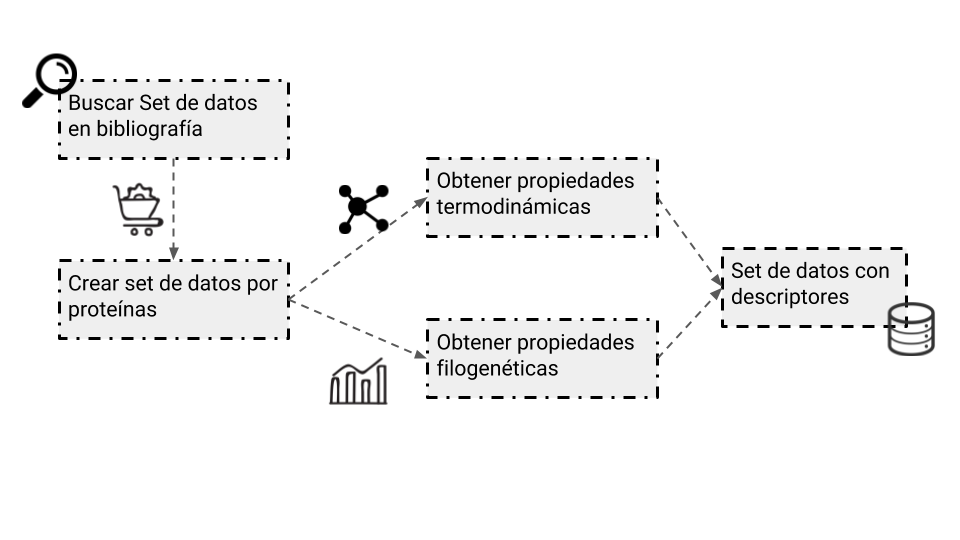
\includegraphics[scale=.4]{m1.png}
	\caption{Esquema representativo asociado al proceso de generación de set de datos de mutaciones puntuales en proteínas.}
	\label{C2:M1}
\end{figure}

Tal como se expone en la Figura \ref{C2:M1}, los set de datos se buscan en la bibliografía, a partir de modelos desarrollados previamente, bases de datos, en la literatura, etc. El objetivo fundamental, es encontrar proteínas con mutaciones puntuales cuyo efecto sea conocido, dicha respuesta puede ser categórica, es decir, asociada al diseño e implementación de modelos de clasificación o continua y se aplica para modelos de regresión. 

En una segunda instancia, a partir de la data recolectada, ésta se procesa con el fin de poder obtener set de datos de proteínas individuales con una cantidad de ejemplos considerables que permitan el diseño de modelos válidos, para ello, fueron implementados scripts bajo el lenguaje de programación Python con el fin de recuperar las proteínas, obtener la información y generar la data de manera individual, además, eliminar ejemplos ambiguos. Es decir, filas con los mismos valores pero cuya columna de respuesta fuese diferente. 

A partir de esto, se forman $n$ set de datos asociados a $n$ proteínas, cada uno con $m$ ejemplos y cuyos descriptores consisten en el residuo original, posición en proteína, residuo mutado y la respuesta asociada. El desbalance de clases se analiza con respecto a las posibles categorías existentes en la respuesta y el porcentaje de representatividad que éstas poseen en la muestra. Se considera que el set de datos exhibe este comportamiento cuando presentan las características expuestas en la sección \ref{problemas}. En el caso de detectar esta problemática, el conjunto de datos será tratado empleando el método SMOTE (Synthetic Minority Oversampling Technique) \cite{chawla2002smote}.

Posteriormente, se aplican las herramientas SDM \cite{Pandurangan2017} y MOSST \cite{Olivera-Nappa2011} con el fin de obtener los descriptores asociados a las propiedades termodinámicas y filogenéticas, respectivamente. Para ello, scripts implementados en lenguaje de programación Python, son desarrollados para consumir los servicios de dichas herramientas y registrar los resultados obtenidos, formando así, set de datos con los descriptores planteados en los objetivos iniciales. Un punto importante a destacar, es que el uso de SDM implica que las proteínas a trabajar, deben presentar una estructura 3D reportada en el Protein Data Bank \cite{berman2000protein} o al menos poseer un modelo representativo y validado. Esto es debido a que se utilizan informaciones de coordenadas para la estimación del efecto de la mutación, minimizaciones energéticas y estabilización de la mutante.

Ya con los descriptores formados, las características asociadas a variables categóricas son codificadas. Si la totalidad de posibles categorías supera el 20\% del total de características en el set de datos, se aplica Ordinal Encoder, en caso contrario, One Hot Encoder \cite{pedregosa2011scikit}. Ordinal Encoder consiste en la transformación de variables categóricas en arreglos de números enteros con valores desde $0,...,n-1$ para $n$ posibles categorías. Por otro lado, One Hot Encoder, consiste en agregar tantas columnas como posibles categorías existan en el set de datos completadas mediante binarización de elementos (0 si la característica no se presencia, 1 en caso contrario)\footnote{Más detalles sobre la codificación de variables categóricas y secuencias lineales de proteínas serán tratadas en el capítulo \ref{cap3}.}.

Es importante mencionar, que las respuestas asociadas a las mutaciones pueden ser del tipo continuo o categórico, lo cual implica que tanto los modelos como las métricas varían. No obstante, se aplica la metodología indistintamente, con el fin de demostrar la robustez del método y la eficacia de éste sin importar el tipo de modelo que se éste entrenando.

\subsection{Implementación de meta modelos de clasificación/regresión}

La implementación de meta modelos consiste en la obtención de un grupo de estimadores que en conjunto, permiten clasificar o predecir nuevos ejemplos. Para ello, se diseña e implementa una metodología inspirada en Sistemas de Meta Learning y aplicando técnicas estadísticas para la evaluación del desempeño y el uso del meta modelo con nuevos ejemplos.

En la Figura \ref{C2:M2}, se exponen las etapas asociadas a la implementación de meta modelos, contemplando desde la fase de entrenamiento de los modelos hasta la unión en meta clasificadores, lo cual se reporta en la herramienta MLSTools (Paper en redacción). 

Cada una de las etapas, contempla un conjunto de scripts implementados en lenguaje de programación Python y empleando la librería Scikit-Learn para el entrenamiento y evaluación de los clasificadores o predictores \cite{pedregosa2011scikit}, así como Numpy para el uso de módulos estadísticos \cite{doi:10.1109/MCSE.2011.37}.


\begin{figure}[!h]
	\centering
	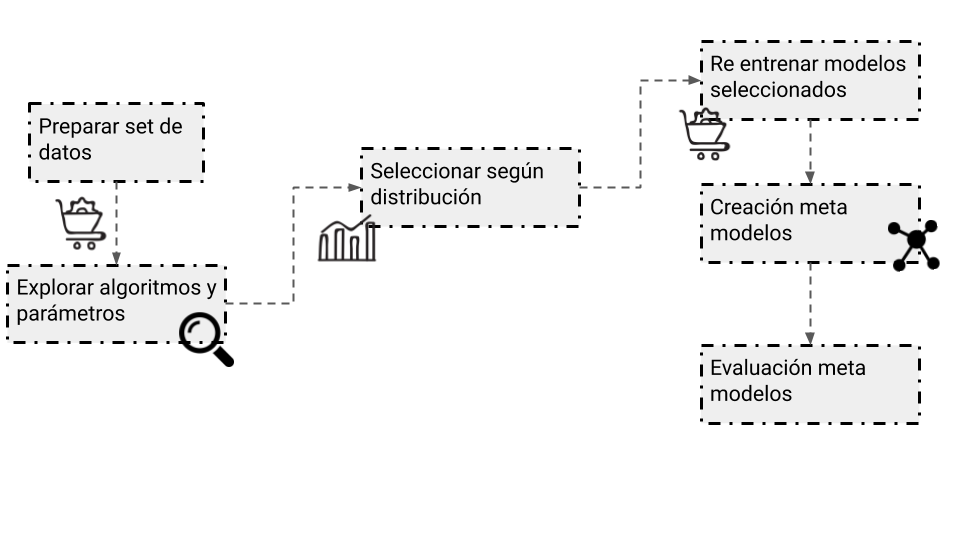
\includegraphics[scale=.4]{m2.png}
	\caption{Esquema representativo asociado al proceso de creación de meta modelos utilizando la metodología reportada para la herramienta MLSTools (Paper en redacción).}
	\label{C2:M2}
\end{figure}

Tal como se observa en la Figura \ref{C2:M2}, es posible identificar etapas claves en el proceso: Exploración de modelos, Selección y Generación de los meta clasificadores/predictores, junto con su evaluación. Cada una de estas etapas se exponen a continuación.

\subsubsection{Exploración de modelos}

La exploración de modelos o estimadores, se basa en la aplicación de diferentes algoritmos de aprendizaje supervisado con variaciones en sus parámetros de configuración inicial. La utilización de los algoritmos, depende principalmente del tipo de respuesta que presente el set de datos, es decir, si es continua o categórica. No obstante, a modo resumen, en la Tabla \ref{cap2:tab1} se exponen los algoritmos utilizados, el caso en el que se usan y los parámetros que se varían junto con el total de iteraciones posibles para cada elemento:

\begin{longtable}[c]{llll|l|l|}
	\hline
	\multicolumn{6}{|c|}{\textbf{Algoritmos y parámetros empleados en la etapa de Exploración en MLSTools}}                                                                                                                                                                                                                                                                                               \\ \hline
	\endfirsthead
	%
	\endhead
	%
	\multicolumn{1}{|l|}{\textbf{\#}} & \multicolumn{1}{l|}{\textbf{Algoritmo}}                                                  & \multicolumn{1}{l|}{\textbf{Tipo}}    & \textbf{Parámetros}                                                                                                                 & \textbf{Uso}                                                         & \textbf{Iteraciones} \\ \hline
	\multicolumn{1}{|l|}{1.}          & \multicolumn{1}{l|}{Adaboost}                                                            & \multicolumn{1}{l|}{Ensamble}         & \begin{tabular}[c]{@{}l@{}}Algoritmo\\ Número estimadores\end{tabular}                                                              & \begin{tabular}[c]{@{}l@{}}Clasificación \\ y Regresión\end{tabular} & 16                   \\ \hline
	\multicolumn{1}{|l|}{2.}          & \multicolumn{1}{l|}{Bagging}                                                             & \multicolumn{1}{l|}{Ensamble}         & \begin{tabular}[c]{@{}l@{}}Bootstrap\\ Número estimadores\end{tabular}                                                              & \begin{tabular}[c]{@{}l@{}}Clasificación y\\ Regresión\end{tabular}  & 16                   \\ \hline
	\multicolumn{1}{|l|}{3.}          & \multicolumn{1}{l|}{\begin{tabular}[c]{@{}l@{}}Bernoulli\\ Naive Bayes\end{tabular}}     & \multicolumn{1}{l|}{Probabilístico}   & Default                                                                                                                             & Clasificación                                                        & 1                    \\ \hline
	\multicolumn{1}{|l|}{4.}          & \multicolumn{1}{l|}{Decision Tree}                                                       & \multicolumn{1}{l|}{Características}  & \begin{tabular}[c]{@{}l@{}}Criterio división\\ Función de impureza\end{tabular}                                                     & \begin{tabular}[c]{@{}l@{}}Clasificación y\\ Regresión\end{tabular}  & 4                    \\ \hline
	\multicolumn{1}{|l|}{5.}          & \multicolumn{1}{l|}{\begin{tabular}[c]{@{}l@{}}Gaussian\\ Naive Bayes\end{tabular}}      & \multicolumn{1}{l|}{Ensamble}         & Default                                                                                                                             & \begin{tabular}[c]{@{}l@{}}Clasificación y\\ Regresión\end{tabular}  & 1                    \\ \hline
	\multicolumn{1}{|l|}{6.}          & \multicolumn{1}{l|}{\begin{tabular}[c]{@{}l@{}}Gradient\\ Tree Boosting\end{tabular}}    & \multicolumn{1}{l|}{Ensamble}         & \begin{tabular}[c]{@{}l@{}}Función de pérdida\\ Número estimadores\end{tabular}                                                     & \begin{tabular}[c]{@{}l@{}}Clasificación y\\ Regresión\end{tabular}  & 16                   \\ \hline
	\multicolumn{1}{|l|}{7.}          & \multicolumn{1}{l|}{\begin{tabular}[c]{@{}l@{}}k-Nearest\\ Neighbors\end{tabular}}       & \multicolumn{1}{l|}{Distancias}       & \begin{tabular}[c]{@{}l@{}}Número Vecinos\\ Algoritmo\\ Métrica distanciaPesos\end{tabular}                                         & \begin{tabular}[c]{@{}l@{}}Clasificación y\\ Regresión\end{tabular}  & 160                  \\ \hline
	\multicolumn{1}{|l|}{9.}          & \multicolumn{1}{l|}{\begin{tabular}[c]{@{}l@{}}Nu Support\\ Vector Machine\end{tabular}} & \multicolumn{1}{l|}{Kernel}           & \begin{tabular}[c]{@{}l@{}}Kernel\\ Nu\\ Grado polinomio\end{tabular}                                                               & \begin{tabular}[c]{@{}l@{}}Clasificación y\\ Regresión\end{tabular}  & 240                  \\ \hline
	\multicolumn{1}{|l|}{10.}         & \multicolumn{1}{l|}{Random Forest}                                                       & \multicolumn{1}{l|}{Ensamble}         & \begin{tabular}[c]{@{}l@{}}Número estimadores\\ Función de impureza\\ Bootstrap\end{tabular}                                        & \begin{tabular}[c]{@{}l@{}}Clasificación y\\ Regresión\end{tabular}  & 32                   \\ \hline
	\multicolumn{1}{|l|}{11.}         & \multicolumn{1}{l|}{\begin{tabular}[c]{@{}l@{}}Support\\ Vector Machine\end{tabular}}    & \multicolumn{1}{l|}{Kernel}           & \begin{tabular}[c]{@{}l@{}}Kernel\\ C\\ Grado polinómio\end{tabular}                                                                & \begin{tabular}[c]{@{}l@{}}Clasificación y\\ Regresión\end{tabular}  & 240                  \\ \hline
	&                                                                                          &                                       &                                                                                                                                     & \textbf{Total Iteraciones}                                           & \textbf{726}        \\ \cline{5-6} 
	\caption{Tabla resumen, algoritmos implementados, parámetros utilizados e iteraciones involucradas por cada algoritmo.}
	\label{cap2:tab1}\\
\end{longtable}

Como se observa en la Tabla \ref{cap2:tab1}, son sobre 720 modelos los que se generan y a partir de ellos se obtiene distribuciones de medidas de desempeño que permiten evaluarlos. En el caso de modelos de regresión se utilizan los coeficientes de Pearson, Spearman, Kendall $\tau$ y $R^{2}$, mientras que para modelos de clasificación, se consideran la Precisión, Exactitud, Recall y F1.

Finalmente, esta etapa, entrega set de modelos entrenados y evaluados según las métricas de interés. Se destaca que cada modelo es validado a través del proceso de validación cruzada, con el fin de poder disminuir posibles sobreajustes. El valor de $k$ asociado a las subdivisiones a realizar varía con respecto a la cantidad de ejemplos que presente el set de datos, es decir, sea $n$ la cantidad de ejemplos en la muestra, si $n<=20$ se tiene que $k=n$ implicando el uso de Leave one out, si $n>20$ y $n<=50$ se considera un valor de $k=3$, si $n>50$ y $n<=100$ $k=5$, por último, si $n>100$ se tiene un valor de $k=10$.

\subsubsection{Selección de modelos}

Cada distribución de medida de desempeño perteneciente a los modelos entrenados en la fase de Exploración, se somete a test estadísticos basados en Z-score \cite{pedregosa2011scikit} que permite seleccionar los modelos cuyas métricas representen outliers positivos dentro de la distribución.

El algoritmo general, utilizado para el desarrollo de esta selección es como se expone en el algoritmo \ref{alg:select}, para el cual se detallan los pasos simplificados que permiten obtener un conjunto de modelos entrenados y que representan los valores más altos dentro de su distribución. Es importante mencionar, que se obtiene un conjunto $M'$ con los modelos, considerando como punto de selecciones los valores evaluados con respecto a la desviación estándar, considerando los umbrales 3 $\sigma$, 2 $\sigma$ y 1.5 $\sigma$ por sobre la media, si ningún factor se cumple, sólo se considera el valor máximo en la distribución.

Es importante mencionar, que cada distribución puede permitir la selección de distintos modelos, lo cual implica que un mismo modelo pueda ser seleccionado en diferentes medidas, razón por la cual, a la hora de obtener el conjunto de modelos $M'$ se remueven aquellos elementos que se encuentran repetidos. Siendo estos, sólo los modelos que presenten igualdad tanto en el algoritmo como en sus parámetros de configuración inicial.

\begin{algorithm}[H]
	\begin{algorithmic}[1]
		\REQUIRE Conjunto $M$ con modelos entrenados y sus medidas de desempeño, Lista $L$ con medidas de desempeño. \label{lin:lineaRara}
		\ENSURE Conjunto $M'$ con modelos seleccionados.
		
		
		\FOR{$i$ en $L$} 
		\STATE Calcular  media $\mu$, desviación estándar $\sigma$ en distribución $M_{i}$
		\FOR{$ x \in M_{i}$}
		\IF {$x \ge \mu + 3*\sigma$}
		\STATE Agregar $x$ a $M'$
		\ENDIF
		\ENDFOR
		\IF {largo $M'$ = 0}
		\FOR{$ x \in M_{i}$}
		\IF {$x \ge \mu + 2*\sigma$}
		\STATE Agregar $x$ a $M'$
		\ENDIF
		\ENDFOR
		
		\IF {largo $M'$ = 0}
		\FOR{$ x \in M_{i}$}
		\IF {$x \ge \mu + 1.5*\sigma$}
		\STATE Agregar $x$ a $M'$
		\ENDIF
		\ENDFOR
		
		\IF {largo $M'$ = 0}
		\FOR{$ x \in M_{i}$}
		\IF {$x = MAX{M_{i}}$}
		\STATE Agregar $x$ a $M'$
		\ENDIF
		\ENDFOR
		\ENDIF
		\ENDIF
		\ENDIF
		\ENDFOR
		
		\RETURN $D$ sin valores extremos
	\end{algorithmic}
	\caption{Algoritmo de selección de modelos}\label{alg:select}
\end{algorithm}

\subsubsection{Generación y evaluación de meta modelos}

A partir del conjunto de modelos $M'$, el cual representa los estimadores seleccionados, cuyas medidas de desempeño son las más altas en sus distribuciones correspondientes, se generan meta modelos, es decir, estimadores compuestos de diversas unidades, los cuales en conjunto entregan una respuesta, ya sea por ponderación o votación. El proceso general para la generación de los meta modelos, es descrito a continuación.

En una primera instancia, los modelos son nuevamente entrenados y se comparan las nuevas medidas de desempeño con las obtenidas previamente. En caso de que exista una diferencia mayor al 20\%, en cualquiera de sus métricas, el modelo se remueve del conjunto $M'$. La razón fundamental de esto, es debido a que se espera desarrollar modelos robustos cuyas evaluaciones no presenten variaciones significativas y que realmente no alteren sus predicciones ante nuevos ejemplos, razón por la cual, se aplica nuevamente validación cruzada para validar los modelos.

Con el fin de evaluar el desempeño de los meta modelos, nuevas medidas se generan a partir de la información resultante de los modelos individuales. No obstante, la forma en la que se obtienen varían dependiendo del tipo de respuesta que se debe entregar.

Si la respuesta es continua, se obtiene los valores de predicción de cada modelo y se promedian, para luego aplicar las métricas estándar (Coeficiente de Pearson, Kendall $\tau$, Spearman y $R^{2}$) sobre estos valores promediados y los reales. Expresado matemáticamente:

Sea $M'$ la cantidad de elementos en el meta modelo, $n$ la cantidad de ejemplos en el set de datos y sea $Y$ el vector de respuestas reales de tamaño $n$. Para cada $M'_{i}\ \in\ M'$ se obtiene un vector $Y_{i}$ que representa los valores de predicción entregados por el modelo $M'_{i}$. A partir de cada $Y_{i}$ se genera una matriz de predicciones $P(mxn)$ donde $m$ representa la cantidad de modelos en $M'$. Finalmente, se obtiene un vector $Y'$ de tamaño $n$, el cual se compone de la media de cada columna en la matriz $P$, es decir, para el ejemplo $i$ se obtienen $m$ predicciones, las cuales son promediadas, formando el valor $Y'_{i}\ \in\  Y'$. Vector el cual, se utiliza para obtener las métricas de desempeño.

Para el caso en que la respuesta sea categórica, es decir, los modelos son del tipo clasificación, se obtiene la respuesta de cada modelo individual y se selecciona una única categoría, correspondiente a aquella que presente una mayor probabilidad de ocurrencia dada la distribución de elementos y considerando para ello las probabilidades iniciales de cada categoría en el set de datos de estudio. De esta forma, se obtiene un vector respuesta con la clasificación de cada ejemplo cuyo valor corresponde al evento más probable a ocurrir, este vector se compara con el set de respuestas reales y se aplican las métricas de interés para clasificadores.

\subsection{Cómo usar los meta modelos para la clasificación de nuevos ejemplos?}

Nuevos ejemplos pueden ser clasificados o predecir su respuesta, dependiendo sea el caso, a partir de los meta modelos desarrollados. En el caso de estimadores basados en variables continuas, los nuevos ejemplos se someten a cada uno de los modelos individuales pertenecientes al sistema, los cuales generan una respuesta individual, a partir de dichas respuestas, se genera un intervalo de confianza con un nivel de significancia $\alpha=0.01$ donde existe una mayor probabilidad de que se encuentre el valor real de la predicción dado los valores del entrenamiento. Para ejemplos que impliquen clasificación, se obtiene la respuesta de cada modelo individual y se evalúa la probabilidad de ocurrencia de cada categoría, entregando así, la respuesta condicionada por una probabilidad de ocurrencia del evento.

\subsection{Uso de meta modelos en sistemas de proteínas}

El objetivo principal de esta metodología, radica en el hecho de crear una herramienta que permita implementar modelos basados en algoritmos de aprendizaje supervisado para set de datos de mutaciones puntuales o variantes para una misma proteína. 

Un flujo general del uso de la herramienta, se expone en la Figura \ref{C2:M3}.

\begin{figure}[!h]
	\centering
	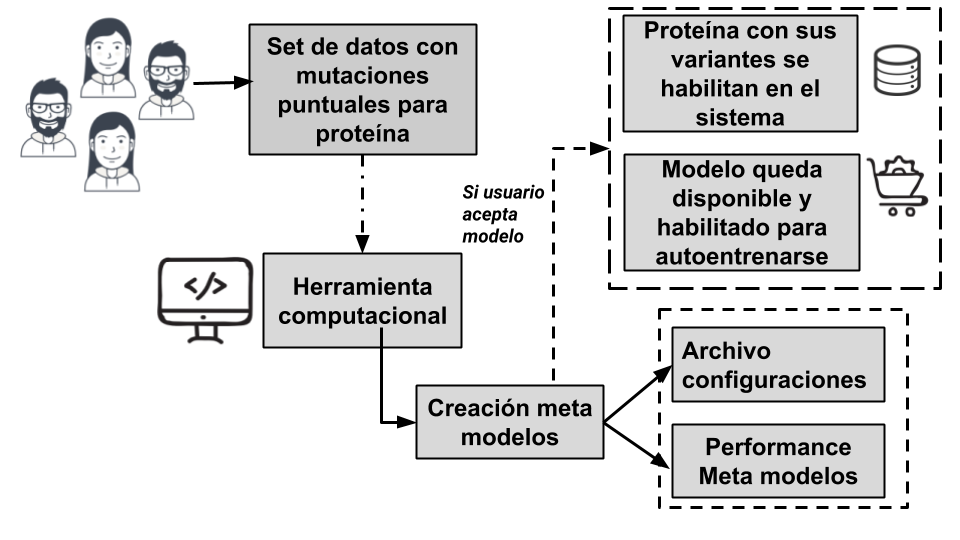
\includegraphics[scale=.4]{m3.png}
	\caption{Esquema representativo de flujo asociado a la herramienta de generación de meta modelos para mutaciones puntuales en proteínas de interés.}
	\label{C2:M3}
\end{figure}

La idea general, consiste en que usuarios de la herramienta, puedan entrenar sus propios modelos de clasificación o regresión, basados en la metodología expuesta en los pasos anteriores mediante el uso de Meta Learning Sytem Tools (Paper en Redacción). Para ello, los usuarios deben entregar sus set de datos con la información necesaria para ser procesada: cadena, residuo original, posición, residuo mutado y respuesta o efecto de la mutación, además del archivo PDB a ser procesado. 

La herramienta, aplica los pasos expuestos en la metodología de este capítulo generando un meta modelo basado en algoritmos de aprendizaje supervisado y las medidas de desempeño que permiten evaluar el modelo obtenido. 

Si el usuario acepta la metodología y permite la publicación de los datos, el sistema habilita el acceso tanto a los meta modelos como a los set de datos y los agrega a la lista de procesos de modelos auto entrenables.

Esto último, implica que ante la adición de nuevos ejemplos al set de datos, el sistema actualiza los modelos y las medidas de desempeño, aplicando la metodología expuesta, así, constantemente mantiene la actualización de la información y permite mantener en constante crecimiento los datos que contemplan el desarrollo de los modelos.

\section{Análisis y evaluación de los set de datos a utilizar}

A continuación, se exponen los resultados obtenidos hasta el momento, presentando principalmente, los set de datos a utilizar, las características que estos poseen y qué representan, con el fin de contextualizar la data a manipular y los modelos a generar.

\subsection{Set de datos utilizados}

En el presente apartado se describen las características básicas de los set de datos trabajados, así como también, qué representan las proteínas bajo las cuales se están desarrollando los modelos de estimadores.

\subsubsection{Descripción general}

Los set de datos utilizados, tanto para la formación de los inputs asociados al sistema, así como también la validación de respuesta correspondiente a la mutación que estos tienen, fueron extraídos desde distintas bases de datos de mutaciones en proteínas de estudios relacionados a los cambios que provoca la sustitución del residuo inicial, ya sea a nivel de cambios energéticos o estabilidad de la proteína.

11 set de datos con respuesta continua fueron obtenidos. Cada set de datos contemplaba como elemento a predecir, las diferencias de energía libre de Gibbs, entre los residuos originales y mutados. Las mutaciones fueron seleccionadas desdes diversos estudios en los cuales se reportaron, centrándose en \cite{Wainreb2011, Sun2017, petukh2016saambe, Alexov2012,prot20185}.

Adicional a los set de datos con respuesta continua, 8 conjuntos de elementos asociados a tareas de clasificación fueron obtenidos desde diversos estudios reportados a la actualidad \cite{ancien2018prediction, broom2017computational, capriotti2008three, quan2016strum, Capriotti2005, 1gzp030, Khan2010, masso2008accurate, getov2016saafec}. 

De tal manera, se generó un total de 19 conjuntos de set de datos, con respuesta categórica y continua, los cuales se asocian a proteínas independientes, usadas para la evaluación de las metodologías planteadas. Estas 19 proteínas junto con su descripción, se exponen en la Tabla \ref{cap2:tab2}.


\begin{longtable}[c]{|l|l|l|l|l|}
	\hline
	\multicolumn{5}{|c|}{\textbf{Resumen set de datos de proteínas y sus características}}                                                                                                                                                                                             \\ \hline
	\endfirsthead
	%
	\endhead
	%
	\textbf{\#} & \textbf{Código PDB} & \textbf{Tipo} & \textbf{Ejemplos} & \textbf{Descripción}                                                                                                                                                                                       \\ \hline
	1.          & 1A22                & Regresión     & 132               & \begin{tabular}[c]{@{}l@{}}Human growth hormone bound to single\\ receptor\end{tabular}                                                                                                                    \\ \hline
	2.          & 1CH0                & Regresión     & 191               & \begin{tabular}[c]{@{}l@{}}Crystal and molecular structures of the complex\\ of alpha-*Chymotrypsin with its inhibitor Turkey\\ Ovomucoid third domain\end{tabular}                                        \\ \hline
	3.          & 1DKT                & Regresión     & 119               & \begin{tabular}[c]{@{}l@{}}CKSHS1: Human cyclin dependent\\ kinase subunit, type 1 complex with\\ metavanadate\end{tabular}                                                                                \\ \hline
	4.          & 1FKJ                & Regresión     & 219               & \begin{tabular}[c]{@{}l@{}}Atomic structure of FKBP12-FK506, \\ an immunophilin  immunosupressant\\ complex\end{tabular}                                                                                   \\ \hline
	5.          & 1FTG                & Regresión     & 203               & \begin{tabular}[c]{@{}l@{}}Structure of apoflavodoxin: closure of\\ a Tyr/Trp aromatic gate leads to a\\ compact fold\end{tabular}                                                                         \\ \hline
	6.          & 1PPF                & Regresión     & 190               & \begin{tabular}[c]{@{}l@{}}X-Ray crystal structure of the complex\\ of human leukocyte elastase and the\\ third domain of the Turkey ovomucoid\\ inhibitor\end{tabular}                                    \\ \hline
	7.          & 1RX4                & Regresión     & 556               & \begin{tabular}[c]{@{}l@{}}Dihydrofolate reductase (E.C.1.5.1.3) complexed\\ with 5,10-Dideazatetrahydrofolate and\\ 2'-Monophosphadenosine 5'-Diphosphoribose\end{tabular}                                \\ \hline
	8.          & 1WQ5                & Regresión     & 239               & \begin{tabular}[c]{@{}l@{}}Crystal structure of tryptophan synthase\\ alpha-subunit from Escherichia coli\end{tabular}                                                                                     \\ \hline
	9.          & 2AFG                & Regresión     & 134               & Human acidic fibroblast growth factor                                                                                                                                                                      \\ \hline
	10.         & 3SGB                & Regresión     & 191               & \begin{tabular}[c]{@{}l@{}}Structure of the complex of Streptomyces\\ Griseus protease B and the Third domain\\ of the Turkey ovomucoid inhibitor\end{tabular}                                             \\ \hline
	11.         & 5AZU                & Regresión     & 203               & \begin{tabular}[c]{@{}l@{}}Crystal structure analysis of oxidize\\ Pseudomonas Aeruginoa Azurin at PH 5.5\\ and PH 9.0. A PH-induced conformational\\ Transition involves a peptide bond flip\end{tabular} \\ \hline
	12.         & 1BN1                & Clasificación & 1802              & Carbonic anhydrase II inhibitor                                                                                                                                                                            \\ \hline
	13.         & 1BVC                & Clasificación & 561               & \begin{tabular}[c]{@{}l@{}}Structure of a Biliverdin Apomyoglobin\\ complex\end{tabular}                                                                                                                   \\ \hline
	14.         & 1LZ1                & Clasificación & 848               & \begin{tabular}[c]{@{}l@{}}Human Lysozyme. Analysis of Non-Bonded\\ and Hydrogen-Bond interactions\end{tabular}                                                                                            \\ \hline
	15.         & 1STN                & Clasificación & 2193              & \begin{tabular}[c]{@{}l@{}}The crystal structure of Staphylococcal\\ Nuclease\end{tabular}                                                                                                                 \\ \hline
	16.         & 1VQB                & Clasificación & 820              & \begin{tabular}[c]{@{}l@{}}Gene V Protein (Single-Stranded DNA\\ Binding Protein)\end{tabular}                                                                                                             \\ \hline
	17.         & 2CI2                & Clasificación & 741               & \begin{tabular}[c]{@{}l@{}}Crystal and molecular structure of the\\ Serine proteinase inhibitor CI-2 from\\ Barley seeds\end{tabular}                                                                      \\ \hline
	18.         & 2LZM                & Clasificación & 2336              & Structure of Baceriophage T4 Lysosyme                                                                                                                                                                      \\ \hline
	19.         & 2RN2                & Clasificación & 712               & \begin{tabular}[c]{@{}l@{}}Structural details of ribonuclease H from\\ Escherichia Coli\end{tabular}                                                                                                       \\ \hline
	\caption{Resumen de proteínas utilizadas para el desarrollo de meta modelos basados en metodología Meta Learning System propuesta durante este capítulo.}
	\label{cap2:tab2}\\
\end{longtable}

Cada una de las proteínas presentan diferentes características y funcionalidades, algunas facilitan la unión a DNA, mientras que otras presentan propiedades enzimáticas, por otro lado, existen enzimas que representan inhibidores, entre las principales. Esto es interesante a la hora de evaluar el poder que presenta la metodología con respecto al análisis de diferentes proteínas, estructuras y complejos, ya que se presenta una gran variedad en cuanto a forma y funcionalidad de éstas, lo que implica que el sistema no se limita por cierto tipo de estructuras o complejos.

A modo de ilustrar las diferencias estructurales de las proteínas en estudio, en la Figura \ref{fig:proteins} se exponen algunas de las estructuras asociadas a las proteínas utilizadas para desarrollar modelos de clasificación o regresión.

\begin{figure}
	\centering
	\begin{subfigure}{0.4\textwidth}
		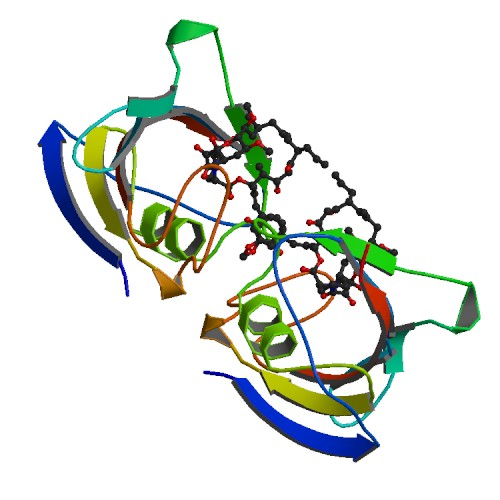
\includegraphics[width=\textwidth]{1fkj.jpg}
		\caption{1FKJ}
		\label{fig:1FKJ}
	\end{subfigure}
	~ %add desired spacing between images, e. g. ~, \quad, \qquad, \hfill etc. 
	%(or a blank line to force the subfigure onto a new line)
	\begin{subfigure}{0.4\textwidth}
		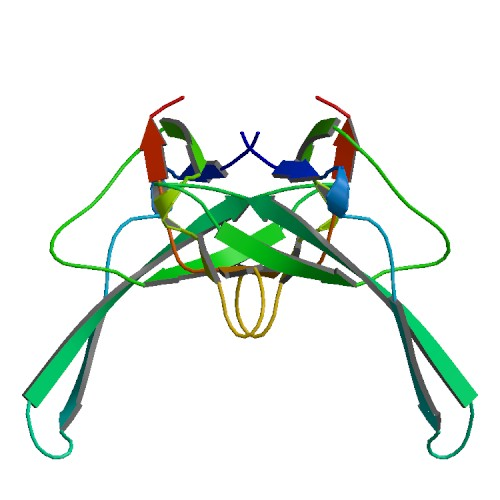
\includegraphics[width=\textwidth]{1vqb.jpg}
		\caption{1VQB}
		\label{fig:1VQB}
	\end{subfigure}
	~ %add desired spacing between images, e. g. ~, \quad, \qquad, \hfill etc. 
	%(or a blank line to force the subfigure onto a new line)
	\begin{subfigure}{0.4\textwidth}
		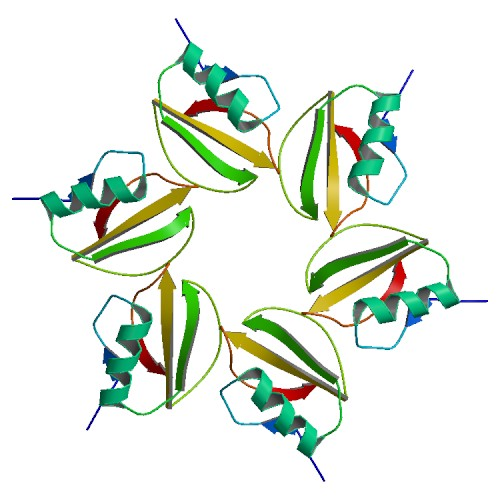
\includegraphics[width=\textwidth]{2ci2.jpg}
		\caption{2CI2}
		\label{fig:2CI2}
	\end{subfigure}
	
	\begin{subfigure}{0.4\textwidth}
		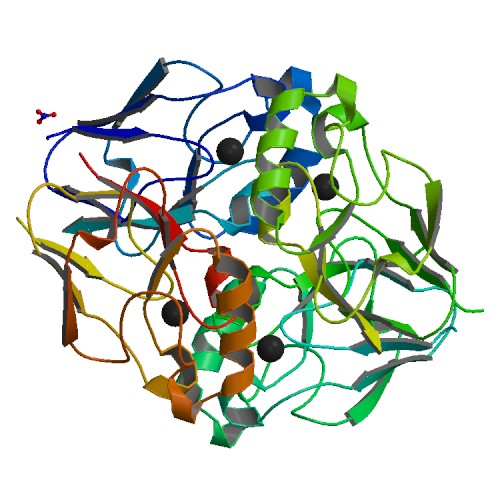
\includegraphics[width=\textwidth]{5azu.jpg}
		\caption{5AZU}
		\label{fig:5AZU}
	\end{subfigure}
	\caption{Representación de estructuras de proteínas ejemplos utilizadas para el desarrollo de meta modelos de clasificación.}
	\label{fig:proteins}
\end{figure}

Las mutaciones fueron recolectadas desde diferentes set de datos, por lo que, en caso de información ambigua, es decir, una misma mutación con diferentes respuestas, no fueron consideradas. Por otro lado, debido a que para la aplicación de la herramienta SDM se necesitaba la cadena a la cual pertenece en residuo, scripts desarrollados en Python y utilizando la librería BioPython, permitieron procesar los archivos asociados a las estructuras de las proteínas, identificadas desde el Protein Data Bank (PDB) \cite{abola1984protein}. Descartando aquellas mutaciones reportadas en las que no se encontró la cadena, obteniendo como resultante la cantidad de mutaciones reportadas para cada proteína expuestas en la Tabla \ref{cap2:tab2}.

\subsubsection{Evaluación del desbalance de clases y distribución de respuestas continuas}

El desbalance de clases se evaluó en aquellos set de datos con respuesta categórica, lo cual contempla, tres posibles casos: Neutral, Estable, No Estable, esto es debido a que todos los estudios donde se evalúan mutaciones, normalmente se analizan cambios que alteren la estabilidad de la proteína. En la Figura \ref{fig:desbalance}, se aprecia a modo ejemplo dos set datos y su distribución de categorías para la variable respuesta.

\begin{figure}[!h]
	\centering
	\begin{subfigure}{0.8\textwidth}
		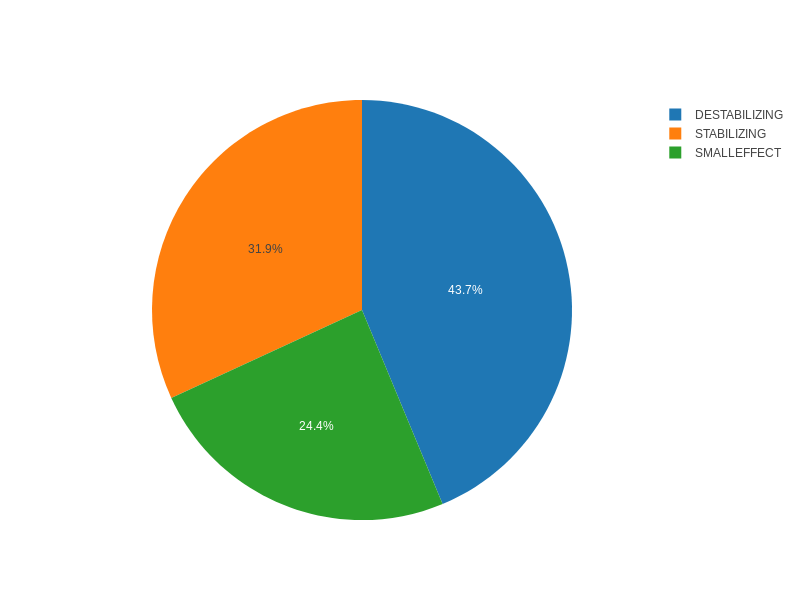
\includegraphics[width=\textwidth]{class1STN.png}
		\caption{1STN}
		\label{fig:des1}
	\end{subfigure}
	~ %add desired spacing between images, e. g. ~, \quad, \qquad, \hfill etc. 
	%(or a blank line to force the subfigure onto a new line)
	\begin{subfigure}{0.8\textwidth}
		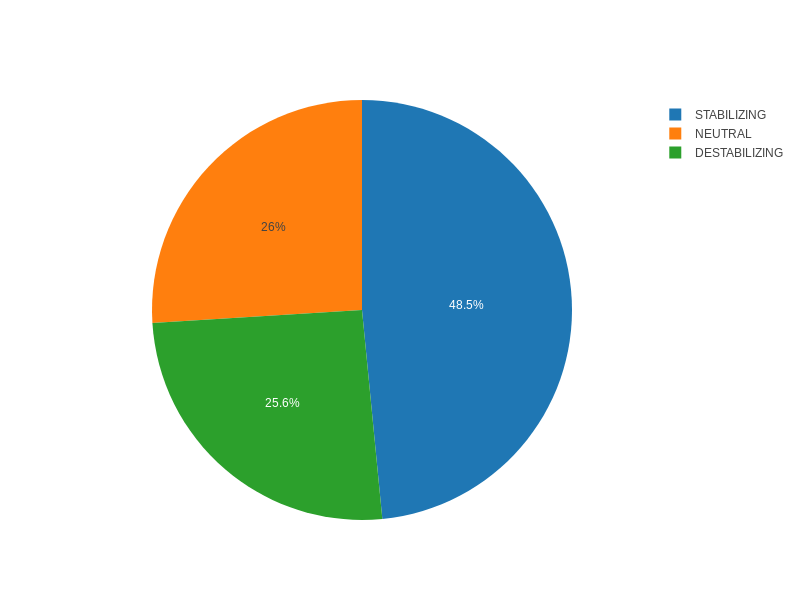
\includegraphics[width=\textwidth]{class2RN2.png}
		\caption{2RN2}
		\label{fig:des2}
	\end{subfigure}
	
	\caption{Evaluación del desbalance de clases en proteínas ejemplo.}
	\label{fig:desbalance}
\end{figure}

En las 8 proteínas en estudio para modelos de clasificación, la distribución de las categorías es similar a lo expuesta en la Figura \ref{fig:desbalance} para todas ellas, donde cerca del 50\% corresponden a mutaciones que afectan positivamente a la estabilidad, mientras que mutaciones que provocan cambios negativos o no generan diferencias, se encuentran en proporciones similares, ambas cercanas al 25\%. 

Si bien las proporciones son dispares, para este caso, se considera un desbalance como un elemento que representa menos de un 5\% del total de la muestra, además, dado a que la cantidad de ejemplos son elevadas, un 20\% o un 25\% implica cerca de 200 mutaciones, en promedio, que cumplen dicha característica. También, el hecho de que exista una cantidad inferior de mutaciones no benéficas a la estabilidad viene dada a la dificultad de encontrar y reportar mutaciones que afecten negativamente a para una proteína, es debido a la propensión filogenética \cite{Olivera-Nappa2011} que estos ocurran, lo cual se ve reflejado en las diferencias asociadas a cambios positivos dentro del set de mutaciones. No obstante, si bien el hecho de que la propensión filogenética indique que el cambio tiende a mejorar estabilidad, diseñar mutantes con mejoras en propiedades de interés, es un problema latente en la actualidad, de alto costo económico y computacional y con una gran demanda desde diferentes áreas del conocimiento.

En los set de datos para el desarrollo de modelos de regresión, se evaluó la distribución de la respuesta, en este caso, valores de $\Delta\Delta\ G$ asociado a diferencias de energía libre producidas entre el residuo mutado y el original, tal que: $\Delta\ Res_{mut}\ - \Delta\ Res_{wild}\ = \Delta\Delta\ G$. 

Las distribuciones se evaluaron utilizando el test de Shapiro, con el fin de determinar si la distribución se comportaba como una normal. Para todas las proteínas estudiadas, en los 11 set de datos, las respuestas presentaron distribución normal, con valores de Shapiro sobre 0.8 y un p-value $\leq$ 0.01, lo cual indica una alta confianza estadística en los resultados presentados por dicho test.

Una visualización de las distribuciones puede generarse a partir del desarrollo de histogramas, los cuales, a modo de ejemplo se expone en la Figura \ref{fig:histogram}.

\begin{figure}[!h]
	\centering
	\begin{subfigure}{0.48\textwidth}
		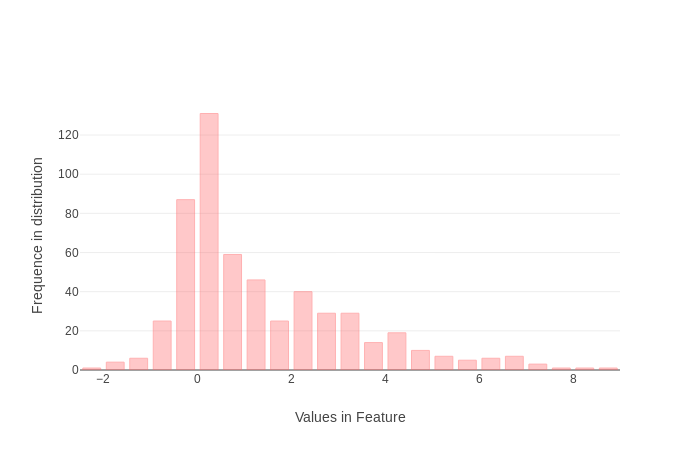
\includegraphics[width=\textwidth]{1RX4.png}
		\caption{Histograma para respuesta continua en 1RX4}
		\label{fig:hist1}
	\end{subfigure}
	~ %add desired spacing between images, e. g. ~, \quad, \qquad, \hfill etc. 
	%(or a blank line to force the subfigure onto a new line)
	\begin{subfigure}{0.48\textwidth}
		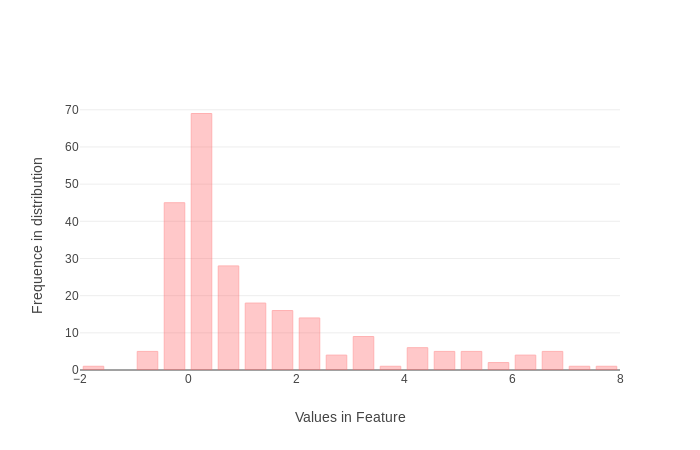
\includegraphics[width=\textwidth]{1WQ5.png}
		\caption{Histograma para respuesta continua en 1WQ5}
		\label{fig:hist2}
	\end{subfigure}
	
	\caption{Evaluación de la distribución de respuesta continua en set de datos de proteínas.}
	\label{fig:histogram}
\end{figure}

El análisis de estas características es relevante a la hora de diseñar modelos de clasificación o regresión, debido a que si existe una tendencia por una clase condiciona al clasificador a \textit{"aprender en base a la mayoría"}, por lo que puede aumentar los errores en cuanto a falsos positivos, dado a que, no se tiene la cantidad de ejemplos suficientes para una clase que permitan al modelo capturar las posibles variaciones asociadas a ésta.

Dado a los análisis de evaluación de representatividad de categorías en el set de datos y distribución de respuestas continuas, se expone que los set de datos seleccionados no presentan desbalance significativo para el caso de desarrollo de modelos de clasificación y a su vez, todas las respuestas asociadas a cambios en la energía libre para modelos de regresión, presentan distribución normal. Razón por la cual, es factible el desarrollo de modelos asociados a las respuestas presenten en los set de datos seleccionados. No obstante, sólo se ha considerado el problema del desbalance y la evaluación de distribución en la respuesta continua, una vez caracterizado los set de datos a partir de las propiedades fisicoquímicas y termodinámicas, se analizarán las características y cómo éstas condicionan la clasificación o la predicción de cambios energéticos.
